\documentclass{article}
\usepackage[a4paper, tmargin=1in, bmargin=1in]{geometry}
\usepackage[utf8]{inputenc}
\usepackage{graphicx}
\usepackage[justification=centering]{caption}

% \usepackage{parskip}
\usepackage{pdflscape}
\usepackage{listings}
\usepackage{hyperref}
\usepackage{caption}
\usepackage{subcaption}
\usepackage{float}
\usepackage{enumerate}
\usepackage{amsmath}

\setlength{\parindent}{0pt}

\title{CS 754 : Advanced Image ProcessingAssignment 2}
\author{Meet Udeshi - 14D070007\\
  Arka Sadhu - 140070011\\
}
\date{\today}

\begin{document}
\maketitle

\section*{Q1}
\subsection*{A1.1}

$$ y = \Phi x, y\in \text{I\!R}^{m}$$

If $m=1$ then $y$ is a single value. Assume $x_i\neq 0$ for some $i \in \{1,...,n\}$
then $y = \Phi_i x_i$.
Consider some other $x'$ which has $j^{\text{th}}$ element non-zero, $j\neq i$.
If $\Phi_j x'_j = \Phi_i x_i$, then $y=\Phi x'$ is also satisfied. We can find
such a $x'$ for all $j\neq i$ where $x'_j = \Phi_i/\Phi_j x_i$.
Hence there is no unique solution for this equation, and we cannot uniquely determine $x$ from
$y$.
\\
\\
For the case where we know the index of the non-zero element in $x$, we have been given
$i$, and no other $j\neq i$ will satisfy the equation, leaving behind only one solution for $x$. Hence now we can uniquely determine $x$ from $y$.

\subsection*{A1.2}

If $m=2$, then $y$ is a 2D vector. Assuming $i$ is the index of non-zero element in
$x$

$$ y = \left[ 
  \begin{array}{c}
    \Phi_{1i}x_i\\
    \Phi_{2i}x_i
  \end{array} 
\right] 
$$

We can say that $y$ is the 2D column vector $\Phi_i$ scaled by $x_i$. Assume no two columns
of $\Phi$ are parallel to each other in 2D space. Then we can say that we will find only
one unique $i$ for which the equation holds. This is because if $y \| \Phi_i$ and
$y \| \Phi_j$, $i\neq j$ then $\Phi_i \| \Phi_j$, which is contrary to our assumption.
\\
\\
If the assumption holds for some $\Phi$, we can obtain $i$ by calculating
normalised dot product of $y$ with every column $\Phi_i$, and whichever $i$ gives
$\frac{y\cdot\Phi_i}{|y||\Phi_i|} = 1$, we can then use it to calculate $x_i$ by

$$x_i = |y|/|\Phi_i| $$

If there are two or more such $i$, we can say that our assumption doesn't hold on $\Phi$ and
no unique solution can be found.

\subsection*{A1.3}

For $m=3$, $y$ is a 3D vector which can be represented as the linear combination
of two columns of $\Phi$. Take $i$ and $j$ to be the two indices of $x$ which are
non-zero.

$$ y = \Phi_i x_i + \Phi_j x_j $$

We can see that $y$ in 3D space will lie in the 2D plane defined by $\Phi_i$ and
$\Phi_j$. So to find $x$ given $y$, we need to find two columns of $\Phi$ which form
$\{\Phi_i,\Phi_j,y\}$ as a set of coplanar 3D vectors. Thus we need to find $i,j$ s.t.

$$ \frac{y\times\Phi_i}{|y||\Phi_i|} = \frac{y\times\Phi_j}{|y||\Phi_j|} $$

We will be able to find a unique pair of $i,j$ iff no three columns of $\Phi$ are coplanar
in 3D.
\\
\\
Algorithm:
\begin{enumerate}
\item{Create a binary search tree to add normalised cross products}
\item{Loop through the columns of $\Phi$ and for every $\Phi_i$
    \begin{enumerate}
    \item{Calculate normalised cross product $\hat{n_i} =  \frac{y\times\Phi_i}{|y||\Phi_i|}$}
    \item{Search for $\hat{n_i}$ in the tree and return both indices,
        current index and matched index if found. Break the loop.}
    \item{If not found, add $\hat{n_i}$ to the tree.}
    \end{enumerate}
  }
\item{Using the two indices we need to solve for $x_i$ and $x_j$ using 
    $$y = (\Phi_i \Phi_j)\left(\begin{array}{c} x_i\\ x_j \end{array}\right) $$
    This is an over-determined system (three equations two variables)
    and we can use inverse to find a solution (by discarding one equation).}
\end{enumerate}

\subsection*{A1.4}
For $m=4$, we proceed in the same way as above. The only change is that now, $y$ lies in the 2d column subspace of
two columns of $\phi$. So we will be able to find $x$ uniquely iff no columns of $\phi$ are coplanar in a 2d plane
defined in $R^4$
Since we. cannot take cross product in 4D space, we proceed differently. For every $(i,j)$ pair, we make a matrix say $B$,
whose columns are $\phi_i$ and $\phi_j$. Now we equate $Bx_1 = y$ where $x_1 = [\alpha | \beta]^t$. Now we use gaussian elimination.
If we get last two rows as 0 in both $B$ as well as $y$, then we have obtained the solution required. $x$ will have non-zero elements
at indices $i,j$ and the value would be $\alpha$ and $\beta$

\section*{Q2}
\subsection*{A2.1}

We have the relation : $$E_u = \sum_{t=1}^TC_t \cdot F_t$$
Consider $$E_1 = C_1 \cdot F_1$$ and suppose that we want to construct it as a matrix product, then we can write it as
$$E_1 = \phi_1 f_1$$ where $\phi_1 = diag(C_1)$ and $f_1 = vec(F_1)$
Hence $$E_u = [\phi_1 | \phi_2 |...| \phi_T] \begin{bmatrix}
  f_1\\ f_2 \\....\\ f_T \end{bmatrix} $$
Therefore $$x = \begin{bmatrix}
  f_1\\ f_2 \\....\\ f_T \end{bmatrix}$$
$$ y = vec(Eu)$$
$$A = [\phi_1 | \phi_2 |...| \phi_T]$$

\subsection*{A2.2}
For T=3
\begin{figure}[H]
  \centering

  \begin{subfigure}[t]{1.0\linewidth}
    \centering
    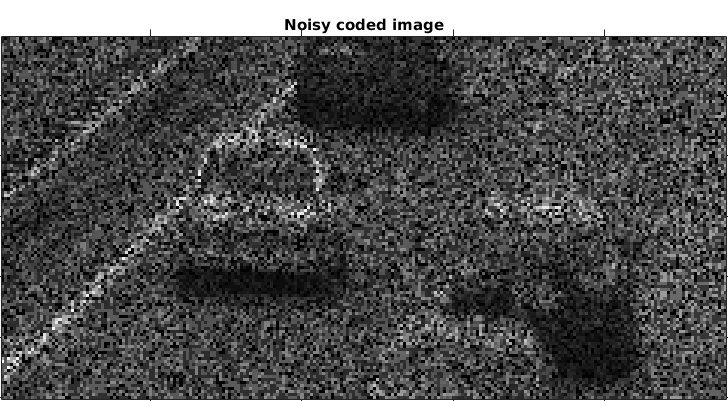
\includegraphics[scale=0.25]{images/noisy_coded_img}
    \caption{Noisy Coded Image}
  \end{subfigure}
  
  
  \begin{subfigure}[t]{1.0\linewidth}
    \centering
    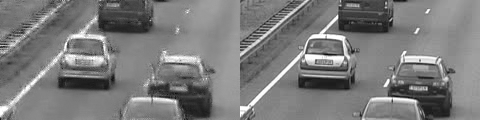
\includegraphics[scale=0.5]{images/frame_1}
      \caption{Frame 1: mse=1.15\%}
  \end{subfigure}
  
  \begin{subfigure}[t]{1.0\linewidth}
    \centering
    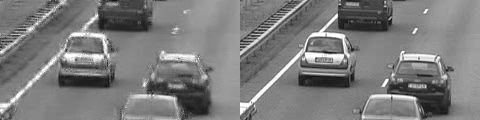
\includegraphics[scale=0.5]{images/frame_2}
      \caption{Frame 2: mse=1.02\%}
  \end{subfigure}
  
  \begin{subfigure}[t]{1.0\linewidth}
    \centering
    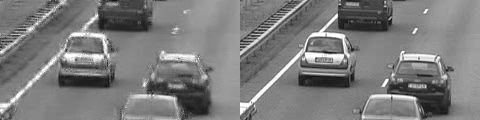
\includegraphics[scale=0.5]{images/frame_2}
    \caption{Frame 3: mse=1.10\%}
  \end{subfigure}
  
  \caption{T = 3}
  \label{fig:1}
\end{figure}
\subsection*{A2.3}
For T=4
\begin{figure}[H]
  \centering

  
  \begin{subfigure}[t]{1.0\linewidth}
    \centering
    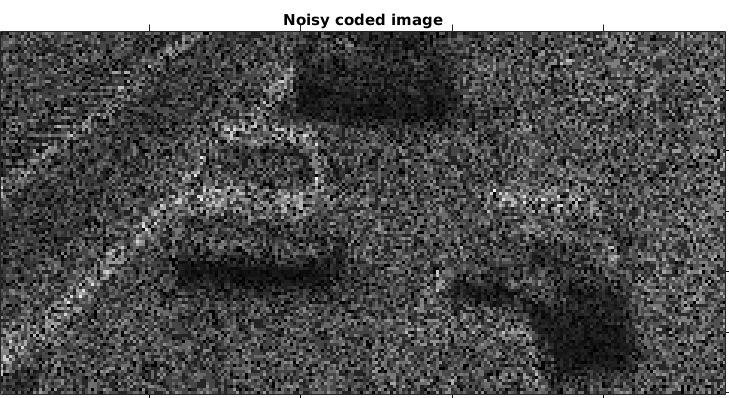
\includegraphics[scale=0.25]{images/noisy_coded_img_t4}
    \caption{Noisy Coded Image}
  \end{subfigure}
  
  \begin{subfigure}[t]{1.0\linewidth}
    \centering
    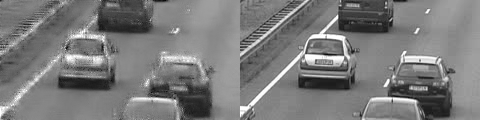
\includegraphics[scale=0.5]{images/frame_1_t4}
      \caption{Frame 1: mse=1.518\%}
  \end{subfigure}

  \begin{subfigure}[t]{1.0\linewidth}
    \centering
    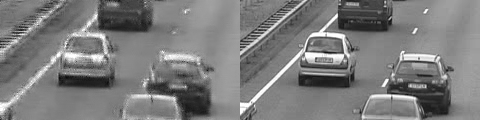
\includegraphics[scale=0.5]{images/frame_2_t4}
    \caption{Frame 2: mse=1.613\%}
  \end{subfigure}

  \begin{subfigure}[t]{1.0\linewidth}
    \centering
    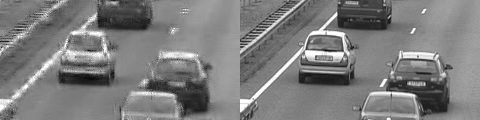
\includegraphics[scale=0.5]{images/frame_3_t4}
    \caption{Frame 3: mse=1.543\%}
  \end{subfigure}

  \begin{subfigure}[t]{1.0\linewidth}
    \centering
    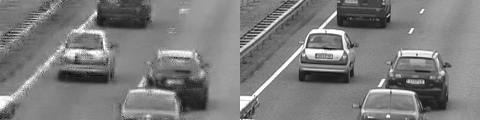
\includegraphics[scale=0.5]{images/frame_4_t4}
    \caption{Frame 4: mse=1.507\%}
  \end{subfigure}
  \caption{T = 4}
\end{figure}






\section*{Q3}
\subsection*{A3}
Coherence is defined as : $$\mu(\phi,\psi) = \sqrt(n)*\max_{i,j \in {0,1,..,n-1}} |\phi^{i^{t}}\psi_j|$$

\begin{enumerate}[(a)]
\item Upper Bound:
  Consider a row of $\phi$ matrix to be exactly same as one of the columns of $\psi$ the inner product would be 1, because both matrices are unit normalized, and result in $\mu_{max}(\phi,\psi) = \sqrt(n)$.
\item Lower Bound:
  Let $g$ be a row of the $\phi$ matrix, which is unit normalized. $g$ can be written with basis vectors as columns of $\psi$. That is
  $$g = \sum_{k=1}^{n}\alpha_k \psi_k$$
  Also since $g$ is unit norm, $$\sum_{k=1}^n\alpha_k^2 = 1$$
  When we take the inner product of $g$ with $\psi_k$, only one $\alpha$ will remain. Now consider the coherence of $g$ and $\psi$. Clearly
  $$\mu(g,\psi) = \sqrt{n} * max(\alpha_j)_{j=1}^n$$ where $\alpha_j$ is corresponds to the jth coefficient. Now we also know that $$max(\alpha_j)_{j=1}^n \ge avg(\alpha_j)_{j=1}^n$$ and equality occurs when all $\alpha_j$ are equal. Hence to get the minimum coherence we need all $\alpha_j$ to be equal and using the previous constraint on unit norm we get $$\alpha_j = \frac{1}{\sqrt{n}}$$. This gives $$\mu_{min}(g,\psi) = 1$$
  This is the bound for all rows, and hence we have obtained $$\mu_{min}(\phi,\psi) = 1$$
\end{enumerate}

\section*{Q4}
\subsection*{A4}
We note that $A$ is a matrix with unit-normalized columns. Now consider a vector $\theta$ which is $S$-sparse, and let $s$ be the support
of the vector $\theta$. Clearly,
$$||A\theta||^2 = ||A_s\theta_s||^2$$
where $A_s$ is constructed by taking only those columns of $A$ corresponding to which $\theta$ is non-zero. The above statement is true
because all other terms of $A\theta$ would be $0$ and wouldn't contribute to the norm.
The maximum and minimum value of $||A_s\theta_s||^2$ will be determined by the largest and smallest singular values. And singular values are basically eigenvalues of the matrix $A_s^tA_s$. Therefore,
$$\lambda_{min}||\theta_s||^2 \leq ||A_s\theta_s||^2 \leq \lambda_{max}||\theta_s||^2$$ 
where $\lambda_{min}$ and $\lambda_{max}$ are the minimum and maximum eigenvalues of the matix  $A_s^tA_s$.

By Gershgorin's Theorem we have:
$$B_{ii} - r_i < \lambda < B_{ii} + r_i$$ where $B_{ii}$ is the $i^{th}$ diagonal element, and $r_i$ is the sum of absolute values of the off-diagonal elements.\\
Here we consider $B = A_s^tA_s$. Since we have assumed columns of $A$ are unit-normalized, hence the diagonal elements of the matrix $B$
will be $1$. Also we consider the definition of mutual coherence $\mu$
$$\mu(A) = max_{i,j,i \neq j}|A_i \cdot A_j|$$
By this definition it is easy to see that $$r_i \leq \mu * (S-1)$$ because $r_i$ is the sum of absolute off-diagonal elements of the matrix $A_s^tA_s$ and each such element would be less than $\mu$ and at most there can be $S-1$ terms. 
Also by RIP definition we have $$\delta_s = max(\lambda_{max} -1 , 1-\lambda_{min})$$\\
If the first term is larger, we have $\delta_s = \lambda_{max} - 1$.
$$\delta_s < B_{ii} + r_i - 1$$
$$\delta_s < 1 + (S-1)\mu -1$$
$$\delta_s < (S-1)\mu$$
If the second term is larger, we have $\delta_s = 1 - \lambda_{min}$
$$\delta_s < 1 - (B_{ii} - r_i)$$
$$\delta_s < 1 - (1 - (S-1)\mu)$$
$$\delta_s < (S-1)\mu$$

Hence in both cases we have proved that $\delta_s < (S-1)\mu$

\end{document}
